\section{Introduction}

LLMs exhibit a ``jagged" cognitive profile  \cite{DBLP:journals/corr/abs-2510-18212}, excelling at math and reasoning, but deficient in tasks requiring long-term memory, such as interactive assistance or decision-support systems acting over extended interactions~\cite{DBLP:journals/tmlr/GaoGHHJLLQQRWWXZZZXFZLQ26}. In such long-horizon tasks, LLMs are fundamentally constrained by their limited context windows, which restrict their ability to retain interaction history over time \cite{hatalis2023memory}.


To mitigate these limitations, prior work equips LLM agents with external memory systems. Early approaches adopt Retrieval-Augmented Generation (RAG)~\cite{DBLP:conf/nips/LewisPPPKGKLYR020}, where memory access is realized via similarity-based retrieval over unstructured text or embedding stores. Subsequent work introduces more structured memory representations, including hierarchical stores~\cite{DBLP:journals/corr/abs-2510-18866, DBLP:journals/corr/abs-2506-06326} and knowledge graphs (KGs)~\cite{DBLP:journals/corr/abs-2501-13956, DBLP:journals/corr/abs-2502-12110,DBLP:journals/corr/abs-2511-01448}, which explicitly encode entities and relations to support more interpretable and relational retrieval. 
However, retrieval in these systems remains restricted to fixed top-$k$ selection or predefined subgraph traversal, failing to infer new retrieval cues or adapt to intermediate evidence.
Under this formulation, existing memory systems operate as \emph{passive retrieval policies}.


\begin{figure}[t]
    \centering
    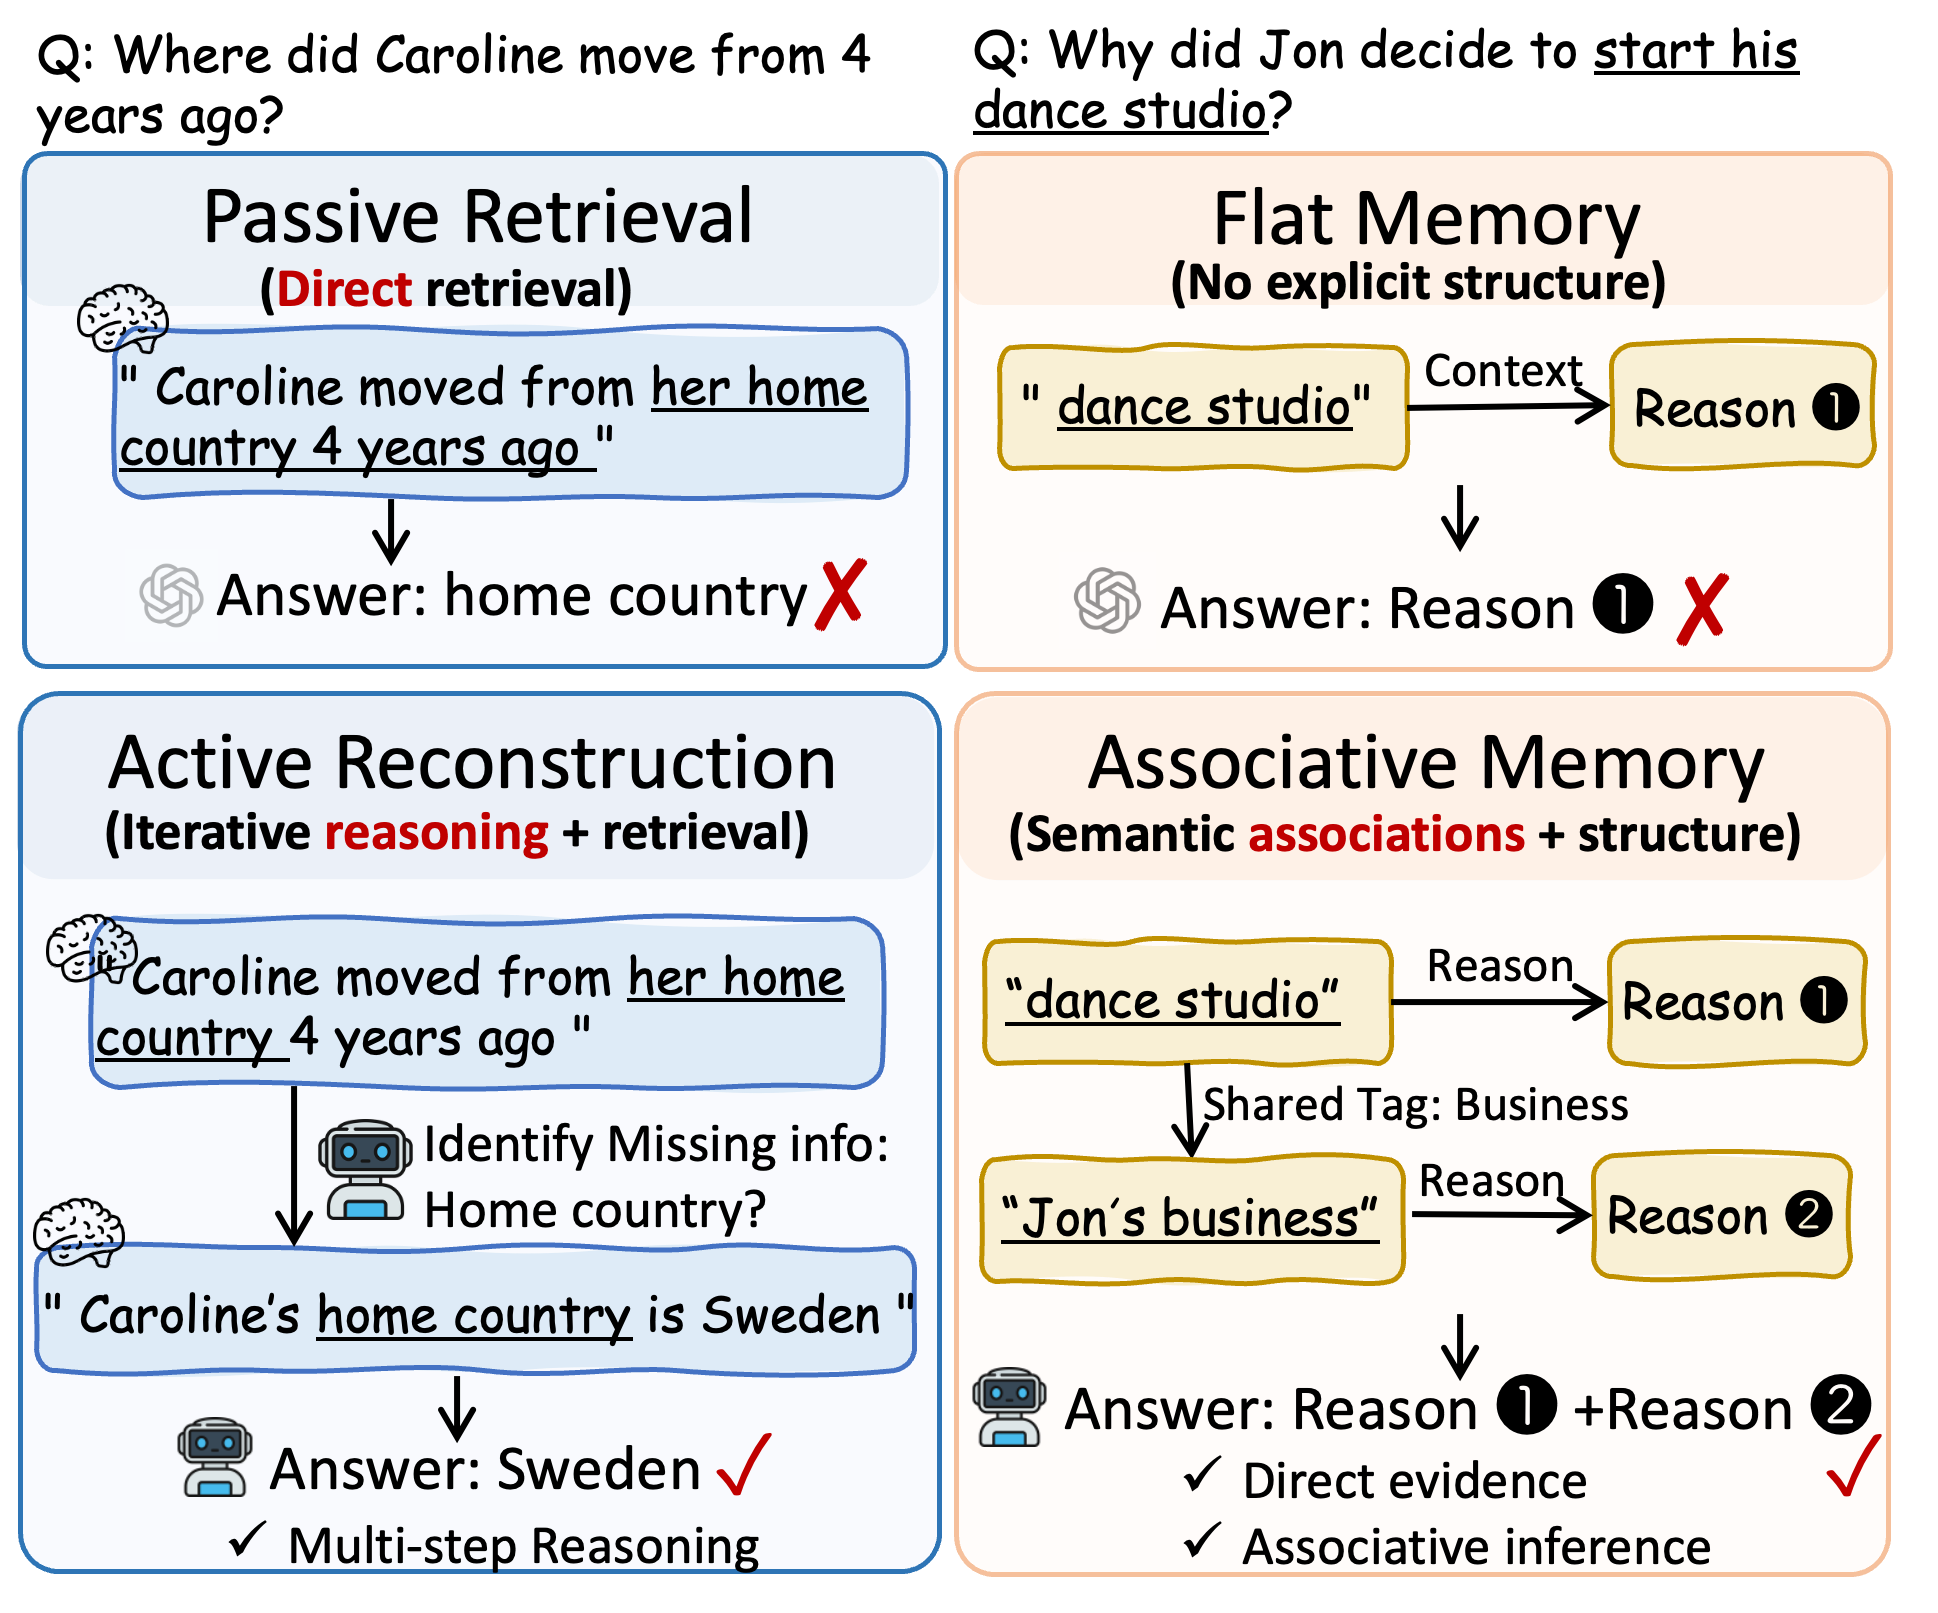
\includegraphics[width=0.9\linewidth]{Fig/fig_intro2.png}
    \caption{Comparison between passive retrieval and active memory reconstruction in MRAgent.}
    \label{fig:introduction}
\end{figure}     
\begin{figure*}[t]
    \centering
    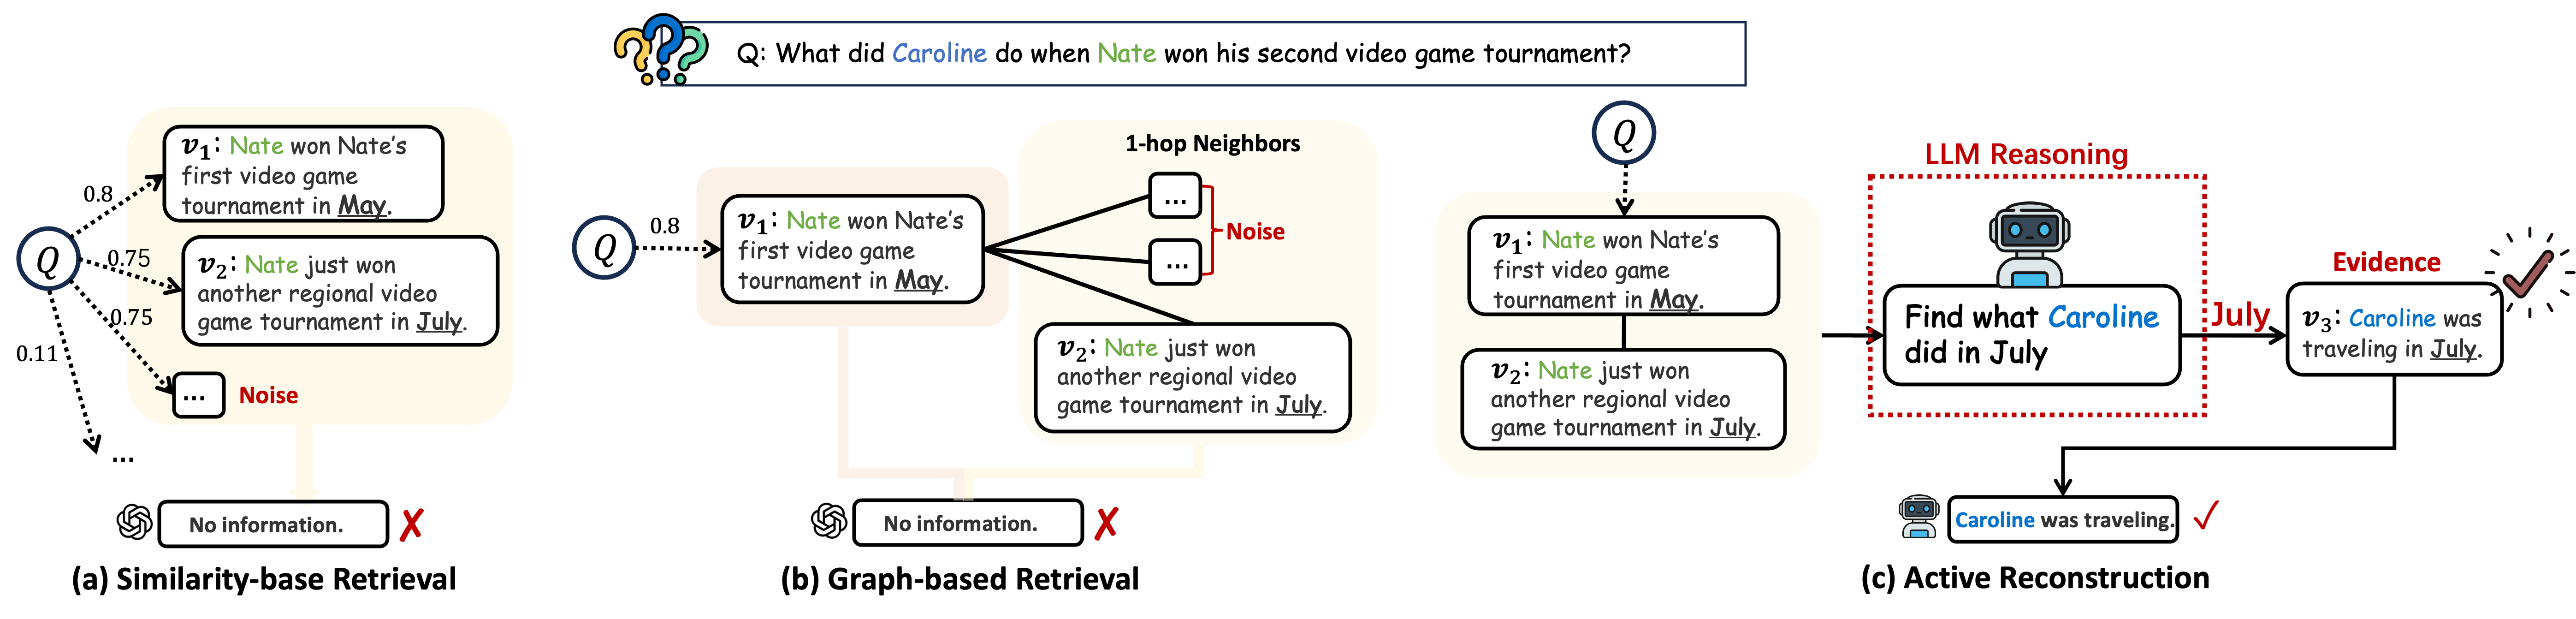
\includegraphics[width=0.95\linewidth]{Fig/fig_motivation.png}
    \caption{
Illustrative example comparing passive retrieval and active reconstruction:
passive retrieval only
retrieves memory content related to Nate’s video game
tournaments based on the query, while active reconstruction infers a critical
temporal cue (``July'') through LLM reasoning and identifies Caroline’s
corresponding activity.
}
    \label{fig:motivation}
\end{figure*}
In contrast, cognitive neuroscience conceptualizes memory retrieval as an \emph{active} and \emph{associative} reconstruction process~\cite{rugg2025cognitive}, rather than a passive read-out of stored content.  
Specifically, retrieval is initiated by contextual cues, which propagate through intermediate representations, progressively reconstructing coherent memory experiences~\cite{frankland2019neurobiological}.

This perspective highlights two key challenges for LLM-based memory systems, as illustrated in Figure~\ref{fig:introduction}.
\textbf{(Challenge 1: Active Reconstruction)} How can memory access be transformed from one-shot retrieval into an active multi-step reconstruction process that progressively reveals information across reasoning steps? \textbf{(Challenge 2: Associative Memory Structure)} How can memory be organized to capture semantic and structural dependencies, enabling guided exploration across associative items? 


In this light, we propose the \textbf{M}emory \textbf{R}easoning Architecture for LLM \textbf{Agent}s (MRAgent), a framework that enables LLM agents to perform active and associative memory reconstruction by integrating LLM reasoning into memory access.
MRAgent explores multiple candidate retrieval paths over a memory graph, pruning irrelevant branches based on intermediate evidence, and iteratively optimizing for the next step with the highest information gain.
To enable controlled memory traversal, we design a Cue–Tag–Content memory graph, where tags encode associations between fine-grained cues and specific memory contents. By exposing these associations explicitly, tags allow the LLM to select retrieval paths before accessing detailed memory contents.
%, in contrast to existing approaches that expand memory based on fixed rules or similarity alone.
Our contributions can be summarized as follows:
\begin{itemize}
    \item We propose active memory reconstruction, a new paradigm that integrates memory access into the reasoning process, allowing the agent to dynamically adapt  search strategy based on intermediate evidence.
    \item We introduce a Cue–Tag–Content memory graph in which associative tags mediate retrieval between cues and content, enabling the LLM to identify promising retrieval paths while pruning irrelevant branches.
    \item We provide a theoretical analysis proving that active retrieval policies are strictly more expressive than passive retrieval.
    \item Extensive experiments demonstrate that MRAgent outperforms strong baselines with significantly improved token and runtime efficiency.
\end{itemize}
